%%%%%%%%%%%%%%%%%%%%%%%%%%%%%%%%%%%%%%%%%%%%%%%%%%%%%%%%%%%%%%%%%%%%%%%%%%%%%%%%
%2345678901234567890123456789012345678901234567890123456789012345678901234567890
%        1         2         3         4         5         6         7         8

\documentclass[letterpaper, 10 pt, conference]{ieeeconf}  % Comment this line out if you need a4paper

%\documentclass[a4paper, 10pt, conference]{ieeeconf}      % Use this line for a4 paper
\usepackage{graphicx}
\usepackage{amsmath}
\usepackage{algorithm}
\usepackage{algorithmic}
\usepackage{morefloats}
\usepackage{dblfloatfix}
\usepackage{amssymb}

\newcommand{\zmin}{z_{min}}
\newcommand{\zmax}{z_{max}}
\newcommand{\ddzc}{\ddot{z}_{c}}
\newcommand{\ddzcf}{\ddot{z}_{c,1}}
\newcommand{\ddzcs}{\ddot{z}_{c,2}}
\newcommand{\rcmpd}{x_{cop,d}}
\newcommand{\rcmpr}{x_{cop,r}}
\newcommand{\icpr}{\boldsymbol{\xi}_r}
\newcommand{\icp}{\boldsymbol{\xi}}
\newcommand{\icpe}{\xi_{x,e}}
\newtheorem{lem}{Lemma}
\graphicspath{{figures/}}
\IEEEoverridecommandlockouts                              % This command is only needed if 
                                                          % you want to use the \thanks command

\overrideIEEEmargins                                      % Needed to meet printer requirements.

%In case you encounter the following error:
%Error 1010 The PDF file may be corrupt (unable to open PDF file) OR
%Error 1000 An error occurred while parsing a contents stream. Unable to analyze the PDF file.
%This is a known problem with pdfLaTeX conversion filter. The file cannot be opened with acrobat reader
%Please use one of the alternatives below to circumvent this error by uncommenting one or the other
%\pdfobjcompresslevel=0
%\pdfminorversion=4

% See the \addtolength command later in the file to balance the column lengths
% on the last page of the document

% The following packages can be found on http:\\www.ctan.org
%\usepackage{graphics} % for pdf, bitmapped graphics files
%\usepackage{epsfig} % for postscript graphics files
%\usepackage{mathptmx} % assumes new font selection scheme installed
%\usepackage{times} % assumes new font selection scheme installed
%\usepackage{amsmath} % assumes amsmath package installed
%\usepackage{amssymb}  % assumes amsmath package installed

\title{\LARGE \bf
Balancing using Vertical Center Of Mass Motion: \\ A 2D Analysis from Model to Robot
%Vertical Center of Mass Motion for Balance Control: Capture Regions and Push Recovery on NASA's Valkyrie
}
\author{Boris J. van Hofslot$^{1,2}$, Robert Griffin$^1$, Sylvain Bertrand$^1$, and Jerry Pratt$^1$% <-this % stops a space
\thanks{This work was supported by NASA's Johnson Space Center under Grant 80NSSC18M0071.}% <-this % stops a space
\thanks{$^{1}$The author is with the Florida Institute for Human and Machine Cognition, 40 S Alcaniz St, 32502 Pensacola FL, United States
        {\tt\small \{bvanhofslot, rgriffin, sbertrand, jpratt\}@ihmc.us}}%
\thanks{$^{2}$The author is with the Department of Cognitive Robotics, Delft University of Technology, Mekelweg 2, 2628 CD Delft, Netherlands
        {\tt\small b.j.vanhofslot@student.tudelft.nl}}%
}


\begin{document}



\maketitle
\thispagestyle{empty}
\pagestyle{empty}


%%%%%%%%%%%%%%%%%%%%%%%%%%%%%%%%%%%%%%%%%%%%%%%%%%%%%%%%%%%%%%%%%%%%%%%%%%%%%%%%

%& ABSTRACT
\begin{abstract}
Balancing strategies for humanoid robots often include center of pressure control (`ankle' strategies), change of body angular momentum (e.g., `hip' strategies) and taking a step. In this work, we propose using vertical center of mass motion as an additional input for balance control. We walk through the process of analyzing simple 2D models, after which we analyze the effects of those models after application on a real robot. First, we specify analytic, theoretical capture regions under unilateral contact and height constraints only. Second, we add a vertical acceleration constraint and come to a simple control law for implementation. Third, we implement the control law in our momentum-based whole-body control framework. We test push recovery while standing on NASA's Valkyrie humanoid robot and compare with a constant height controller, and show that recovery can be improved using vertical motion. Finally, vertical center of mass motion and other balancing strategies are discussed.
\end{abstract}


%%%%%%%%%%%%%%%%%%%%%%%%%%%%%%%%%%%%%%%%%%%%%%%%%%%%%%%%%%%%%%%%%%%%%%%%%%%%%%%%

%% INTRO
\section{INTRODUCTION}
Keeping balance is a fundamental problem in humanoid robotics. Throughout the years, many conditions and expressions have emerged for analyzing the ability of the robot to stabilize. Examples are the capture point and capture region \cite{pratt2006capture, koolen2012capturability}, stability regions \cite{stephens2007humanoid}, the divergent component of motion \cite{takenaka2009real} and the boundedness condition \cite{lanari2014boundedness}, which all link to the energetics of the pendulum-based model and its ability to stabilize.

These conditions commonly rely on a linear inverted pendulum (LIP) model, with optionally a mass with inertia to model the robots angular momentum. The LIP model provides fast, closed-form solutions when integrating over time. This results in the center of mass (CoM) height usually to be fixed in the dynamic planning problem. Vertical center of mass motions are considered as pre-defined and deviations from the dynamic model are considered as disturbances. Those disturbances are commonly controlled with `ankle' strategies, i.e., moving the center of pressure (CoP) or pendulum base, and to a lesser extent, with `hip' strategies: change of body angular momentum. These strategies can be generated by using e.g. a momentum-based whole-body control framework \cite{kajita2003resolved, lee2012momentum,koolen2016design}, which determines center of pressure position and angular momentum rate by optimizing between desired momenta and motion objectives.

\begin{figure}[h]\vspace{0.2cm}
      \centering
      \includegraphics[width=3.3in]{modeltoval.png} %modeltorobot2modelvarzvsang4
      \caption{We analyze the dynamics of a variable height inverted pendulum, as well as push recovery on Valkyrie. }
      \label{fig:modeltoval}
\end{figure}

Although the use of a predefined height trajectory has advantages, it can be overly constraining. In cases where traditional balancing strategies are saturated and the robot is in risk of falling, it is interesting to explore additional methods for the robot to recover. Vertical CoM motion can be used to generate additional horizontal force on the CoM, which can improve balance.

Recently, efforts have been made to use vertical CoM motions for balance control. In \cite{koolen2016balance}, an analytic model predictive controller is derived in 2D from the \textit{orbital energy} proposed in \cite{pratt2007derivation}. Regions of attraction for this controller are investigated, as well as limitations on the region in which recovery is possible for a variable height inverted pendulum model under the constraint of unilateral contact only. In \cite{gao2017increase}, different 2D strategies are proposed for multi-step recovery using vertical CoM motion. In \cite{caron2018balance}, a model predictive control law is proposed in 3D using sequential quadratic programming. The authors manage to solve the nonlinear control problem online using a variable height inverted pendulum model. However, applied results on hardware are not shown yet. Also, \cite{koolen2016balance} and \cite{caron2018balance} use a model predictive control-based approach to use vertical motion in balance control. We believe that in application, special care has to be taken to use such methods, as the model used in prediction may differ a lot from the results on the robot.

In this paper, we analyze capture regions of simple 2D models and analyze the results observed on NASA's Valkyrie after application of these models (see Fig. \ref{fig:modeltoval}). We propose capture regions by adding constraints to a base model. We add a contact unilaterality constraint, followed by height constraints, from which we derive analytic capture regions. We add a vertical force constraint and formulate a bang-bang control law on vertical acceleration, after which the solution to a capture region needs to be computed numerically. Furthermore, we analyze the differences of the found regions with the capture point. Finally, we implement the bang-bang control law in our momentum-based control framework \cite{koolen2016design}. We test push-recovery on NASA's Valkyrie \cite{radford2015valkyrie} and compare with a setup that has a constant height objective and only uses CoP. Furthermore, we discuss the differences that we observe when going from a simple model to the robot.

The remainder of the paper is structured as follows. In Section \ref{sec:models}, we give a short overview of balancing strategies  and \textit{capture}. In Section \ref{sec:regions}, we derive capture regions for a pendulum with variable height, which are analyzed and compared with other balancing strategies in Section \ref{sec:comparison}. We test balancing on NASA's Valkyrie by applying pushes in Section \ref{sec:valkyrie}. Finally, in Section \ref{sec:conclusion}, we conclude and give our outlook on balance control for humanoids.

%% MODELS
\section{MODEL \& CAPTURE}\label{sec:models}
Throughout the paper, we disregard stepping and focus on comparing `0-step' capture \cite{koolen2012capturability}. Our goal is to explore the effects of height variation in balancing tasks, and how these compare to constant height control approaches. To consider vertical motions, we use a variable height inverted pendulum model which has the following dynamics:
\begin{equation}
	\ddot{x} = \frac{x}{z}u,
	\label{eq:height}
\end{equation}
where $u=g+\ddot{z}$, $x$ is the position of the point-mass relative to the CoP and $z$ the height of the mass.

In this paper, we use the term capture region \cite{pratt2006capture} to describe the set of CoP locations, where balance can be achieved. Also, the capture point as introduced by Pratt \textit{et al}. is considered, only this is for comparison denoted as:
\begin{equation}
	x_{cp,lip} = \sqrt{\frac{z_0}{g}}\dot{x}_0,
	\label{eq:xcplip}
\end{equation}
where $z_0$ is the initial height and $\dot{x}_0$ the initial horizontal velocity. To avoid confusion, we use the term \textit{capture position} to describe a point where the current state and the resulting trajectory will lead to stability of the pendulum-based model. We denote a capture position as a positive value:
\begin{equation}
	x_{cp}= |x_0|,\quad \text{if} \quad x_f=0 \quad \text{and} \quad \dot{x}_f=0,
	\label{eq:xcp}
\end{equation}
where $x_{cp}$ is the capture position, $x_f$ the final horizontal position and $\dot{x}_f$ the final horizontal velocity. We use an initial horizontal velocity of greater than zero.

%% THEORETIC REGIONS
\section{CAPTURE REGIONS}\label{sec:regions}
This section proposes bounds on the capture position (\ref{eq:xcp}). The dynamics of (\ref{eq:height}) are considered. For simplicity and comparison with the LIP capture point (\ref{eq:xcplip}), we take the initial vertical velocity $\dot{z}_0=0$. In each subsection, we add constraints to come to a more realistic model. 
\subsection{Unilateral Contact Constraint}
 Considering the constraint of contact unilaterality only, the capture region is bounded by the current position and the ballistic touch down point:
\begin{equation}
	x_{cp,unilateral} \in (0, x_{bal}], \quad \forall u \geq 0, 
	\label{eq:xcpuni}
\end{equation}
where $x_{bal}$ is the ballistic touchdown point. This is the location where the point-mass would intersect the ground plane after a free fall, and $x_{cp,unilateral}$ is the capture position under unilateral contact constraint only. The proof for this region is given in \cite{koolen2016balance}. For the zero initial vertical velocity, the ballistic touchdown point reads as:
\begin{equation}
 x_{bal}=t \dot{x}_0=\sqrt{\frac{2z_0}{g}}\dot{x}_0=\sqrt{2}x_{cp,lip}.
 	\label{eq:xbal}
\end{equation}

The region can be interpreted as follows. At an infinitesimally small distance on the side of CoM in the direction of its horizontal velocity, there exists an infinite impact of the leg that stops the horizontal motion of the CoM. On the other side of the region, the leg, without constraints on height, can apply an impact when the mass is at ground height that stops the motion of the mass.
\subsection{Addition of Height Constraints}
We derive capture positions under a minimum and maximum height constraint respectively, to take kinematic limits of the robot into account. We consider impacts of the leg, such that analytic capture positions can be found. 

Preliminary, we temporally set $\dot{z}_0 \neq 0$ to calculate the influence of an impact on $x_{cp,lip}$. We can use this in the next paragraph to derive a capture position under a minimum height constraint. Considering an initial negative vertical velocity $\dot{z}_0<0$ that is driven to zero by a vertical impact, the influence on the LIP capture point is:
\begin{align}
	x_{cp,I} &= \sqrt{\frac{z_0}{g}}\Big(\dot{x}_0 + \frac{x_{cp,I}}{z_0}\dot{z}_0\Big)\\
	&=\frac{z_0}{\sqrt{gz_0}-\dot{z}_0}\dot{x}_0, \label{eq:xcpimpact}
\end{align}
where $x_{cp,I}$ is the impact influenced capture point from an initial impact that results in $\dot{z}=0$.

Under a minimum height constraint, we can find a capture position from which the trajectory `just' touches the constraint. We first let the mass follow the ballistic trajectory, after which it is vertically stopped by the impact influenced capture point:
\begin{equation}
	x_{cp,\zmin} = x_{bal}(\delta \zmin) + x_{cp,I}(\zmin, \dot{z}_{\zmin}),
	\label{eq:xcpzmincomp}
\end{equation}
where $x_{cp,\zmin}$ is the capture position over the minimum height constraint, $x_{bal}(\delta \zmin)$ the horizontal position after the ballistic fall $\delta \zmin = z0-\zmin$ and $x_{cp,impact}(\zmin,\dot{z}_{\zmin}$) is $x_{cp,impact}$ after the ballistic fall. The velocity at the moment the ballistic trajectory hits the constraint is:
\begin{equation}
	\dot{z}_{\zmin} = -\sqrt{2g\delta \zmin},
\end{equation}
where $\dot{z}_{\zmin}$ is the vertical velocity at $z_{min}$. Using (\ref{eq:xcpzmincomp}), (\ref{eq:xbal}) and (\ref{eq:xcpimpact}), the capture position over the minimum height constraint becomes:
\begin{equation}
	x_{cp,\zmin} = \Bigg(\sqrt{\frac{2\delta_{z_{min}}}{g}} + \frac{\zmin}{\sqrt{g \zmin}+\sqrt{2g\delta_{\zmin}}}\Bigg)\dot{x}_0.
\end{equation}

Also under a maximum height constraint, an analytic capture position can be found. We consider a vertical impact by the leg at the initial position $x=x_0$. This impact is of such magnitude that the mass is exactly at the maximum height constraint, if it is at its apex. After the vertical velocity of the mass is driven to zero by gravity, we apply $x_{cp,lip}$. This point reads as:
\begin{equation}
	x_{cp,\zmax} =\bigg(t_{\dot{z}>0} + \sqrt{\frac{\zmax}{g}}\bigg)\dot{x}_{0,I}
	\label{eq:xcpzmaxcomp}
\end{equation} 
where $x_{cp,\zmax}$ is the capture position following the maximum height constraint, $t_{\dot{z}>0}$ is the time $\dot{z}>0$ and $\dot{x}_{0,I}$ is the initial velocity influenced by the impact. The vertical velocity resulting from the impact that lets the mass just touch $\zmax$ is:
\begin{equation}
	\dot{z}_{I} = \sqrt{2g\delta_{\zmax}},
	\label{eq:dzi}
\end{equation}
where $\delta_{\zmax}=\zmax-z_0$. Filling in (\ref{eq:xcpzmaxcomp}) gives:
\begin{equation}
	x_{cp,\zmax} = \bigg(\frac{\dot{z}_I}{g}+\sqrt{\frac{\zmax}{g}}\bigg)\bigg(\dot{x}_0-\frac{x_{cp,\zmax}}{z_0}\dot{z}_I\bigg).
\end{equation}
Bringing $x_{cp,\zmax}$ to the left-hand side and filling in (\ref{eq:dzi}) gives:
\begin{align}
	x_{cp,\zmax}&=\frac{\frac{\dot{z}_I}{g}+\sqrt{\frac{z_{max}}{g}}}{1+\Big(\frac{\dot{z}_I}{g}+\sqrt{\frac{z_{max}}{g}}\Big)\frac{\dot{z}_I}{z_0}}\dot{x}_0\\
	&=\frac{z_0(\sqrt{2\delta_{\zmax}}+\sqrt{\zmax})}{\sqrt{g}(z_0 + 2\delta_{\zmax} + \sqrt{2\zmax \delta_{\zmax}})}\dot{x}_0.
\end{align}

We will show that the capture positions $x_{cp,\zmin}$ and $x_{cp,\zmax}$ are also the outer bounds on the capture region.

%lem
\begin{lem}\label{lem:regionz}
Considering the dynamics of (\ref{eq:height}), $\dot{z}_0=0$, minimum height constraint $\zmin$ and maximum height constraint $\zmax$, $x_{cp,\zmin}$ and $x_{cp,\zmax}$ are the outer bounds on the capture region.
\end{lem}
%proof
\begin{proof}
For any capture position $x_{cp}$, $x\dot{x}<0$ \cite{koolen2016balance} and $0>x_0\geq-x_{bal}$ (\ref{eq:xcpuni}). 
We use that $x \leq 0, \forall t$ and $x\rightarrow 0$ along any trajectory. From (\ref{eq:height}), and $z>0$, it follows that any input $u$ will slow $\dot{x}$ down. Showing that $\frac{x}{z}\rightarrow 0, \forall t$ will prove that $u=0$ for the longest possible time $t$ will lead to the farthest $x_{cp}$, and a maximum $u$ at the earliest possible $t$ will lead to the closest $x_{cp}$. 

For $u=g$, $z$ remains constant and $\frac{x}{z}\rightarrow 0$. For $u>g$, $z$ will grow and $\frac{x}{z}\rightarrow 0$. If $u<g$, we can show with the derivative of $\frac{x}{z}$ that this is always increasing:
\begin{equation}
\frac{d\frac{x}{z}}{dt}= \frac{z\dot{x}-x\dot{z}}{z^2},
\end{equation}
where $x \leq 0$ and $z \dot{x} \geq 0$. Taking the extreme case $u=0$ leads to:
\begin{align}
	z\dot{x}-x\dot{z} &= (z_0 - \frac{1}{2}gt^2)\dot{x}_0 + (x_0 + \dot{x}_0 t)gt\\
	&= (z_0 +\frac{1}{2}gt^2)\dot{x}_0 + x_0gt.
\end{align}
Noting that all terms are positive except for $x_0$, which has the largest negative value for $x_0=-x_{bal}$:
\begin{align}
	(z_0 +\frac{1}{2}gt^2)\dot{x_0} - \sqrt{\frac{2z_0}{g}}\dot{x}_0gt = \dot{x}_0\bigg(\sqrt{\frac{1}{2}g}t - \sqrt{z_0}\bigg)^2,
\end{align}
which is always greater than zero for all $t$.
\end{proof}

In Fig. \ref{fig:capregion}, the discussed capture regions are visualized. The LIP capture point lies inside the height constrained region, which lies inside the unilateral contact constrained region.
\begin{figure}
      \centering
      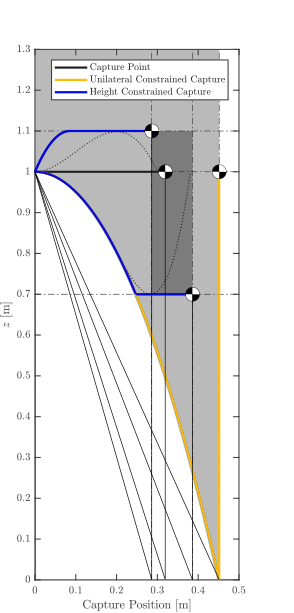
\includegraphics[width=2.3in]{CPLimitsDark.png}
      \caption{Visualization of the analytic capture regions for $\dot{x}_0=1$ and $\dot{z}_0=0$. The light gray area shows the unilateral contact constrained capture region (\ref{eq:xcpuni}). The dark gray area shows the height constrained capture region (Lemma \ref{lem:regionz})  for $0.7<z<1.1$. The dotted plots are made with the \textit{orbital energy controller} of \cite{koolen2016balance} and show that the final points are inside the height constrained region.}
      \label{fig:capregion}
\end{figure}

\subsection{Addition of Vertical Force Constraints}\label{forcecapture}
We can also add constraints on the minimum and maximum vertical force to the dynamics (\ref{eq:height}). In doing so, we assume that the robot specific limitations on joint torques can be approximated with a minimum and maximum vertical acceleration of the CoM. From Lemma 1, any force extremum at the earliest convenience will lead to staying closer to a height constrained bound. By inserting a constraint on vertical acceleration, an analytic solution for a capture position is not available anymore and needs to be solved numerically\footnote[1]{The authors of \cite{gao2017increase} give analytic solutions using vertical acceleration, but consider a constant height in the model. For comparison later in this paper, we do not consider this constant height assumption.}.
     
In \cite{pratt2006capture,stephens2007humanoid,koolen2012capturability}, a bang-bang control law is used to regulate the angular momentum in the body of model. Instead, we use a bang-bang control law on the input $u$ (\ref{eq:height}) to regulate the vertical dynamics:
\begin{multline}
	u = g + \ddot{z}_{c,1}H(t) - (\ddot{z}_{c,1} - \ddot{z}_{c,2})H(t-t_1) \\ - \ddot{z}_{c,2}H(t-t_2),
\end{multline}
where $[\ddzcf,\ddzcs]$ are the first and second constant control inputs and have opposite signs. $H(\cdot)$ is the Heaviside step function and 
\begin{equation}
t_1=\sqrt{\frac{2(z_{const}-z_0)}{\ddzcf - \frac{\ddzcf^2}{\ddzcs}}},
\end{equation}
which is the solution of:
\begin{equation}
	z_0+\frac{1}{2}\ddzcf t_1^2 - \frac{1}{2}\frac{(\ddzcf t_1)^2}{\ddzcs}= z_{const},
\end{equation}
where $z_{const}=\zmin$ if $\ddzcf <0$ and $z_{const}=\zmax$ otherwise. The time $t_2=(1-\frac{\ddzcf}{\ddzcs})t_1$, as the second `bang` needs to drive the vertical velocity resulting from the first bang to zero. We use a binary search to find the capture positions with this control law. In Fig. \ref{fig:zvsf}, simulation results are shown in perspective with the height constrained limits. Note that when the bang-bang control inputs are larger, both trajectory and capture position come closer to the height constrained bounds.
\begin{figure}
      \centering
      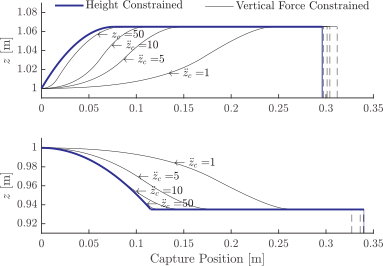
\includegraphics[width=3.3in]{heightvsforcelim2.png}
      \caption{Simulation results for the vertical force constrained capture positions for $\dot{x}_0=1$, $\dot{z}_0=0$ and $\delta \zmax=\delta \zmin=0.065$. The constant acceleration $\ddot{z}_c=|\ddzcf|=|\ddzcs|$ if $\ddot{z}_c \leq g$ and otherwise the constant with negative sign is set to $-g$. The dashed vertical lines mark the capture positions. Closer to the height constrained limit means a higher value of $\ddot{z}_c$.}
      \label{fig:zvsf}
\end{figure}
%% COMPARISON
\subsection{Dimensional Analysis}\label{sec:comparison}
We make a high-level comparison with the LIP, the height constrained bounds and the force constrained capture positions. We use a dimensional analysis as in \cite{pratt2006capture,stephens2007humanoid,koolen2012capturability}. The following parameters are used for dimensionless position and velocity:
\begin{align}
	x' &= \frac{x}{z_0}, \\
	\dot{x}' &= \frac{1}{\sqrt{gz_0}}\dot{x},
\end{align}
In this comparison, we take $\ddzc=|\ddzcf|=|\ddzcs|$ for the vertical force constraint.

For comarison, we make a rough estimate of realistic values of vertical forces that are achievable on both human and robot.

First, we would like to see what would be achievable for a human being. A human jumping vertically with maximum effort generates approximately $2mg$ ground reaction force \cite{linthorne2001analysis}. If we assume this value can also be used in recovery, we can take $\ddot{z}_c=g$ for a human. Second, we want to see what is possible on the robot. We found on hardware experiments on NASA's Valkyrie in Section \ref{subsec:hardware} that $\ddot{z}_c=2.4$ was a well working value. Larger accelerations would result in the robot to shake and did not improve recovery. In Fig. \ref{fig:caplimits}, the height constrained bounds are shown, together with our approximations of what is realistic for vertical acceleration constraints on a human and on the robot. Note how the capture positions relate differently under a minimum height constraint than under a maximum height constraint. Also note how the capture position linking to our approximation for a robot seem to approach a minimum and maximum value quite soon after changing height.
\begin{figure}
      \centering
      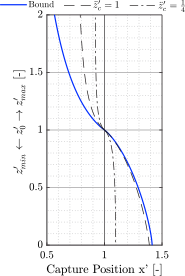
\includegraphics[width=2.2in]{caplimits.png}
      \caption{Plot of reachable dimensionless capture positions for $\dot{x}_0'=1$. }
      \label{fig:caplimits}
\end{figure}

%% VALKYRIE
\section{PUSH RECOVERY ON NASA'S VALKYRIE}\label{sec:valkyrie}
In this section we apply a simple controller that uses vertical motion for balance on Valkyrie while standing. The motivation in control design is, instead of using a model predictive controller, to develop a controller that `gives the best doable` in a worst-case scenario to avoid falling. We compare with CoP control with constant height.
\subsection{Control Law}
Our default control law is based on instantaneous capture point (ICP) \cite{koolen2012capturability} control:
\begin{equation}
	\rcmpd = \rcmpr + k_{\xi}\icpe,
\end{equation}
where $\rcmpd$ is the desired CoP, $\rcmpr$ the reference CoP, $k_{\xi}$ the ICP control gain and $\icpe$ is the ICP error between the reference ICP and the current ICP. For this particular test case we assume a constant $\rcmpr$, in the center of the support polygon. Also, $\rcmpd$ is constrained to be inside the polygon, such that we can make the assumption that no angular momentum is used in recovery.

The robot is controlled with a momentum-based control framework \cite{koolen2016design}. Our framework makes use of \textit{centroidal momentum} \cite{orin2013centroidal}, the angular and linear momentum about the CoM of the robot. 
A desired centroidal momentum rate, along with motion objectives, is sent to a quadratic program, which optimizes over desired joint accelerations and desired ground reaction forces. Desired joint torques are finally computed using an inverse-dynamics algorithm. We typically only select the linear part of the desired momentum rate for control, allowing the controller to use angular momentum rate as needed. The desired horizontal linear momentum rate is computed as:
\begin{equation}
	\dot{\mathbf{l}}_{d,x} = \frac{x-\rcmpd}{z}\big(mg + \dot{\mathbf{l}}_{d,z}\big),
\end{equation}
where $\dot{\mathbf{l}}_{d} \in \mathbb{R}^3$ is the desired linear momentum rate of change. Note that with little vertical motion, $ \dot{\mathbf{l}}_{d,z}$ is small.

Normally while standing, the height is controlled to a default constant reference height. In this experiment, we use a similar control law for vertical acceleration as the bang-bang controller in Section \ref{forcecapture}. The following parameters are used for the controller in addition to the already discussed constraints:
\begin{itemize}
	%\item $\alpha_{\icpe}^+$: Threshold to turn the controller on $|\icpe|>\alpha_{\icpe}^+$, which for example can be tuned to activate the controller when $\rcmpd$ is near the edge of the polygon. 
	%\item $\alpha_{\icpe}^-$: Threshold to turn the controller off $|\icpe|<\alpha_{\icpe}^-$, when the robot is back to stability.
	\item $\dddot{z}_{max}$: maximum allowed vertical CoM jerk.
	\item $\alpha_{\hat{\ddot{z}}_{c}}$: parameter to scale down expected $\ddot{z}_c$ for the second `bang', due to jerk limits.
\end{itemize}

The control sequence we use for the bang-bang controller reads as follows. The controller is activated when the $\rcmpd$ touches the polygon edge, an event that determines the worst-case scenario. The controller turns off if $\icpe$ is at a small value, a measure for stability. For the first `bang': the desired acceleration $\ddot{z}_d=\ddot{z}_c$. The transition from the first `bang' to the second is if:
\begin{equation}
	z+\frac{1}{2}\frac{\dot{z}^2}{\alpha_{\hat{\ddot{z}}_{c}}\ddot{z}_{c}} >\zmax,
\end{equation}
in the case of approaching a maximum height. This results in $\ddot{z}_d=-\ddot{z}_c$ until $\dot{z}<0$, after which the height is controlled to $\zmax$ until the controller turns off:
\begin{equation}
	\ddot{z}_d = k_p(z_r-z)-k_d\dot{z},
\end{equation}
where $[k_p,k_d]=[50.0,14.0]$ are the PD-control gains and reference height $z_r= \zmax$. If the controller is turned off, the height is controlled to the default height and $z_r=z_0$. Finally, $\ddot{z}_d$ is limited with the maximum jerk and $\dot{\mathbf{l}}_{d,z}=m\ddot{z}_d$.
%exp
\subsection{Experimental Setup}
We test push recovery on Valkyrie ($m=127.3$ [kg]) while the robot is standing, by applying a push from the back at chest height. Note that with this setup the resulting motion is always upward, as the CoP is on the other side of the CoM compared to the direction of $\dot{\mathbf{l}}_{d,xy}$. The following parameter values are chosen to work with:
\begin{itemize}
\item $z_0=1.0$ [m], our default reference CoM height during stance.
\item $\zmax=1.065$ [m], the maximum CoM height during stance, such that the legs are not in singular configuration and the feet are still in contact with the ground.
\item $\dddot{z}_{max} = 80.0$ [m/s$^3$].
\item $\ddot{z}_c=2.4$ [m/s$^2$], a value that found to work `well' on hardware. E.g., higher values would result in the robot to shake. 
\end{itemize}

Additionally, whole-body controller parameters relevant to the test are given in Tab. \ref{tab:params}. For the angular motion objectives, the desired is generated with PD-control about a constant reference with $[k_p, k_d]=[100.0,16.0]$. The quadratic program uses an active-set solver \cite{kuindersma2014efficiently}.
\begin{table}[h]
\caption{Relevant whole-body control parameters}
\label{tab:params}
\begin{center}
\begin{tabular}{llc}
\hline~\\[-2ex]
\textbf{Task group} & \textbf{Task} & \textbf{Weight}\\
\hline ~\\[-2ex]
Momentum rate linear& $X$ & $5 \cdot 10^{-2}$\\
Momentum rate linear& $Z$ & $1 \cdot 10^{-2}$\\
Motion angular& Chest $Y$ &    $1.5 \cdot 10^1$\\
Motion angular& Pelvis $Y$ &  $5 \cdot 10^0$\\
Motion angular& Support foot $Y$ &  $5 \cdot 10^0$\\
Regularization & Basis vector multiplier&  $1 \cdot 10^{-5}$\\
Regularization & Basis vector multiplier rate & $5 \cdot 10^{-8}$\\
Regularization & Joint acceleration & $5 \cdot 10^{-3}$\\
Regularization & Joint jerk & $1.6 \cdot 10^{-6}$\\
\hline
\end{tabular}
\end{center}
\end{table}

\subsection{Simulation Results}
For simulation tests, we used a value of $\alpha_{\hat{\ddot{z}}_{c}}=0.4$ for the influence of jerk limitations. We used a push duration of $0.15$ [s], as we were able to apply approximately the same push duration on hardware. We compare our default control setup with the controller that uses vertical motion. 

\subsubsection{Analysis}
The maximum recoverable push for the default control setup is $34.5$ [Ns] for the given push duration. The vertical motion controller still recovered after a push of $37.6$ [Ns]. In Fig. \ref{fig:valcomparephase}, a phase plot is shown for the two push magnitudes for both control setups. The default setup loses stability after the larger push. With the smaller push, the vertical motion controller encircles a considerably smaller area than the default control setup.
\begin{figure}
      \centering
      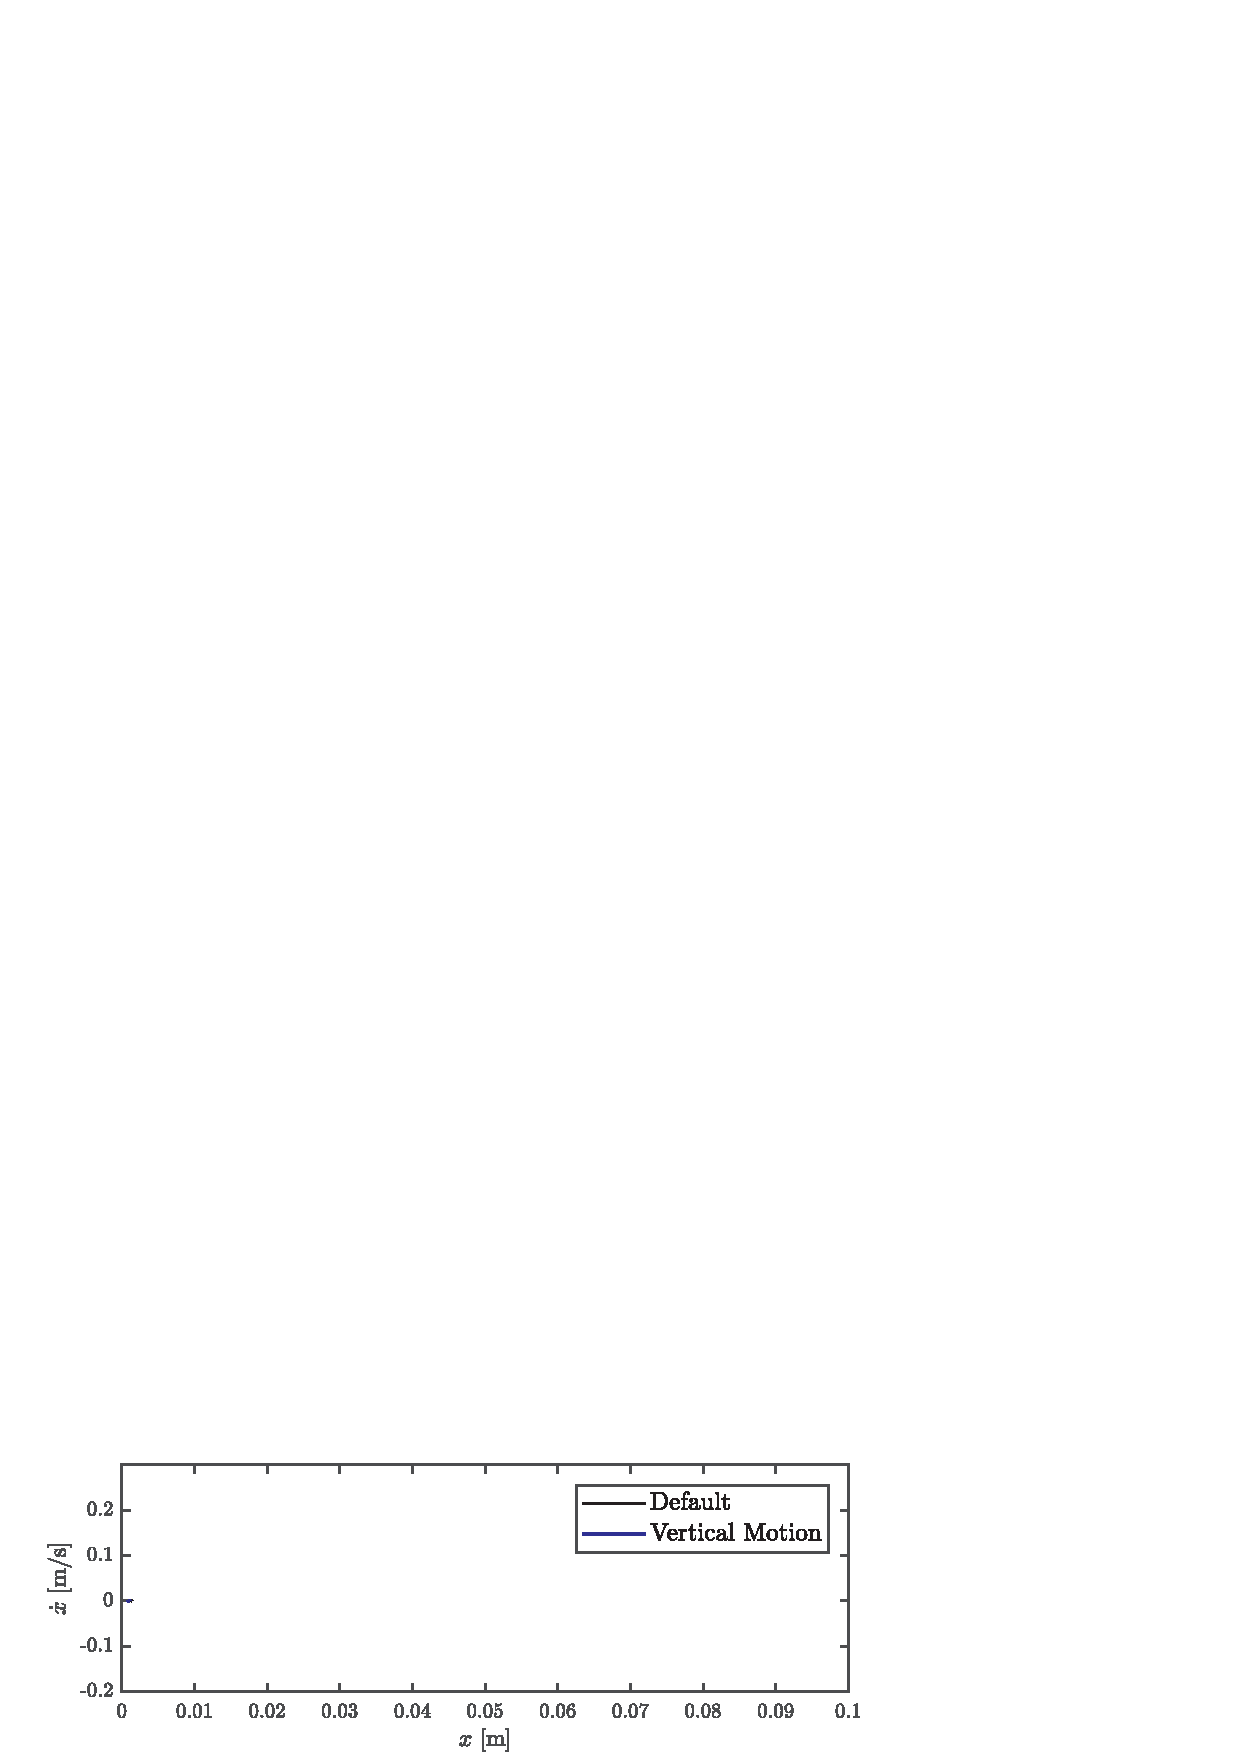
\includegraphics[width=3.3in]{valcomparephase.png}
      \caption{Phase plot of a push of $34.5$ [Ns] (solid) and a push of $37.6$ [Ns] (dotted).}
      \label{fig:valcomparephase}
\end{figure}
\begin{figure}[h]
      \centering
      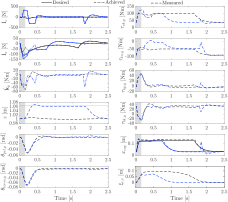
\includegraphics[width=3.3in]{valcomparetime.png}
      \caption{Comparison of push recovery between the default setup (black) versus the vertical motion controller (blue) for a push of $34.5$ [Ns]. The gray area is where the push is applied. `Achieved' is the value after the quadratic program found a solution.}
      \label{fig:valcompare}
\end{figure}

We analyzed the differences in resulting joint torques and noticed that the difference in ankle torque is the largest amount. Furthermore, we found it interesting to compare the maximum rotation error of the pelvis and torso. Angular momentum strategies commonly result in rotation of the upper body. We want to include this rotation in our analysis, as not rotating the body can be one of the advantages of vertical motion compared to angular momentum strategies.

In Fig. \ref{fig:valcompare}, centroidal momentum rate, CoM height and ankle torque plots over time are shown. The achieved vertical linear momentum rates have a little overshoot for both controllers. This may also be a reason for the overshoot in height in the fourth graph in the figure. Conversely, the achieved horizontal linear momentum rate is lower than the desired for both controllers. In the time frame $0.10-0.25$ [s], the vertical motion controller achieves almost double the horizontal momentum rate compared to the default controller. The differences in achieved angular momentum rate are relatively small. We measured a maximum rotation error of $[-0.052,-0.072]$ radians for pelvis and torso respectively for the default setup and $[-0.051,-0.069]$ radians for the vertical motion controller. So the resulting rotation errors in the upper body are even less for the vertical motion controller. The peak ankle torque is higher with the vertical motion controller, but returns to steady-state earlier than the default setup. 


\subsubsection{Comparison with Capture Regions}
The increase in recovery of the vertical motion controller is about $9\%$ compared to the default control setup. The force constrained capture position for the same $\ddot{z}_c$ and $\zmax$ is only about $4\%$ smaller than $x_{cp,lip}$ (see Fig. \ref{fig:caplimits}), which is a remarkable difference compared with the increase in recoverable push. From the results obtained, we assume that a difference in angular momentum is not a reason for this. Also, we noticed that joint angle limits and joint acceleration limits were not violated during the tests. 

However, the difference in the achieved horizontal momentum rate is large. Note that this can be a result of the momentum-based control framework. Generation of horizontal linear momentum rate may conflict with other objectives, such as keeping the upper body straight, and maintaining a certain height. As a side node, we also tried commanding the $\dot{\mathbf{l}}_{d,x}$ of the vertical motion controller, while using $\dot{\mathbf{l}}_{d,z}$ of the default controller, to see if the difference in recovery is just a result of additional desired horizontal linear momentum rate. However, the maximum recoverable push with this setup was the same as with the default setup.

In this case it seemed that the vertical motion controller worked relatively better than expected. Situations where the opposite happens and the controller gives relatively worse results are imaginable as well. If we would have used a model predictive controller for this specific test, it might not have computed at each tick the maximum vertical acceleration possible. With this particular control law for vertical motion we considered in this paper, by determining a worst-case scenario as a logical event, we aimed to produce the maximum available force in the counter direction of the push, while keeping vertical dynamics predictable and horizontal dynamics not.

%% HARDWARE
\subsection{Hardware Results}\label{subsec:hardware}
%\begin{figure}
    %  \centering
  %    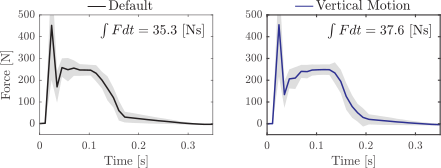
\includegraphics[width=3.3in]{impulsecompare.png}
 %     \caption{Average push force profiles of $12$ pushes where the CoM went closer than $5.0$ [mm] from the polygon edge. %The gray area is the standard deviation above and below the graph. }
 %     \label{fig:impulsecompare}
%\end{figure}
%\begin{figure}
  %    \centering
 %     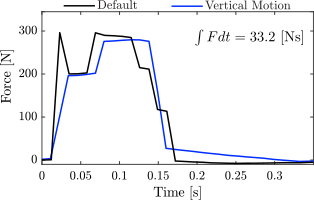
\includegraphics[width=3.3in]{impulse33.png}
 %     \caption{Two push force profiles for both control setups, where the integrated value is the same.}
  %    \label{fig:impulse33}
%\end{figure}
\begin{figure}
      \centering
      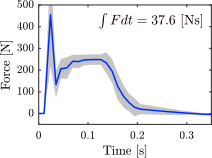
\includegraphics[width=3.3in]{impulsecompare2.png}
      \caption{Average push force profiles of $12$ pushes where the CoM went closer than $5.0$ [mm] from the polygon edge. The gray area is the standard deviation above and below the graph (top). Load sensor on stick with rubber surface (bottom left). Two pushes with approximately the same integrated force (bottom right).}
      \label{fig:impulsecompare}
\end{figure}
\begin{figure}
      \centering
      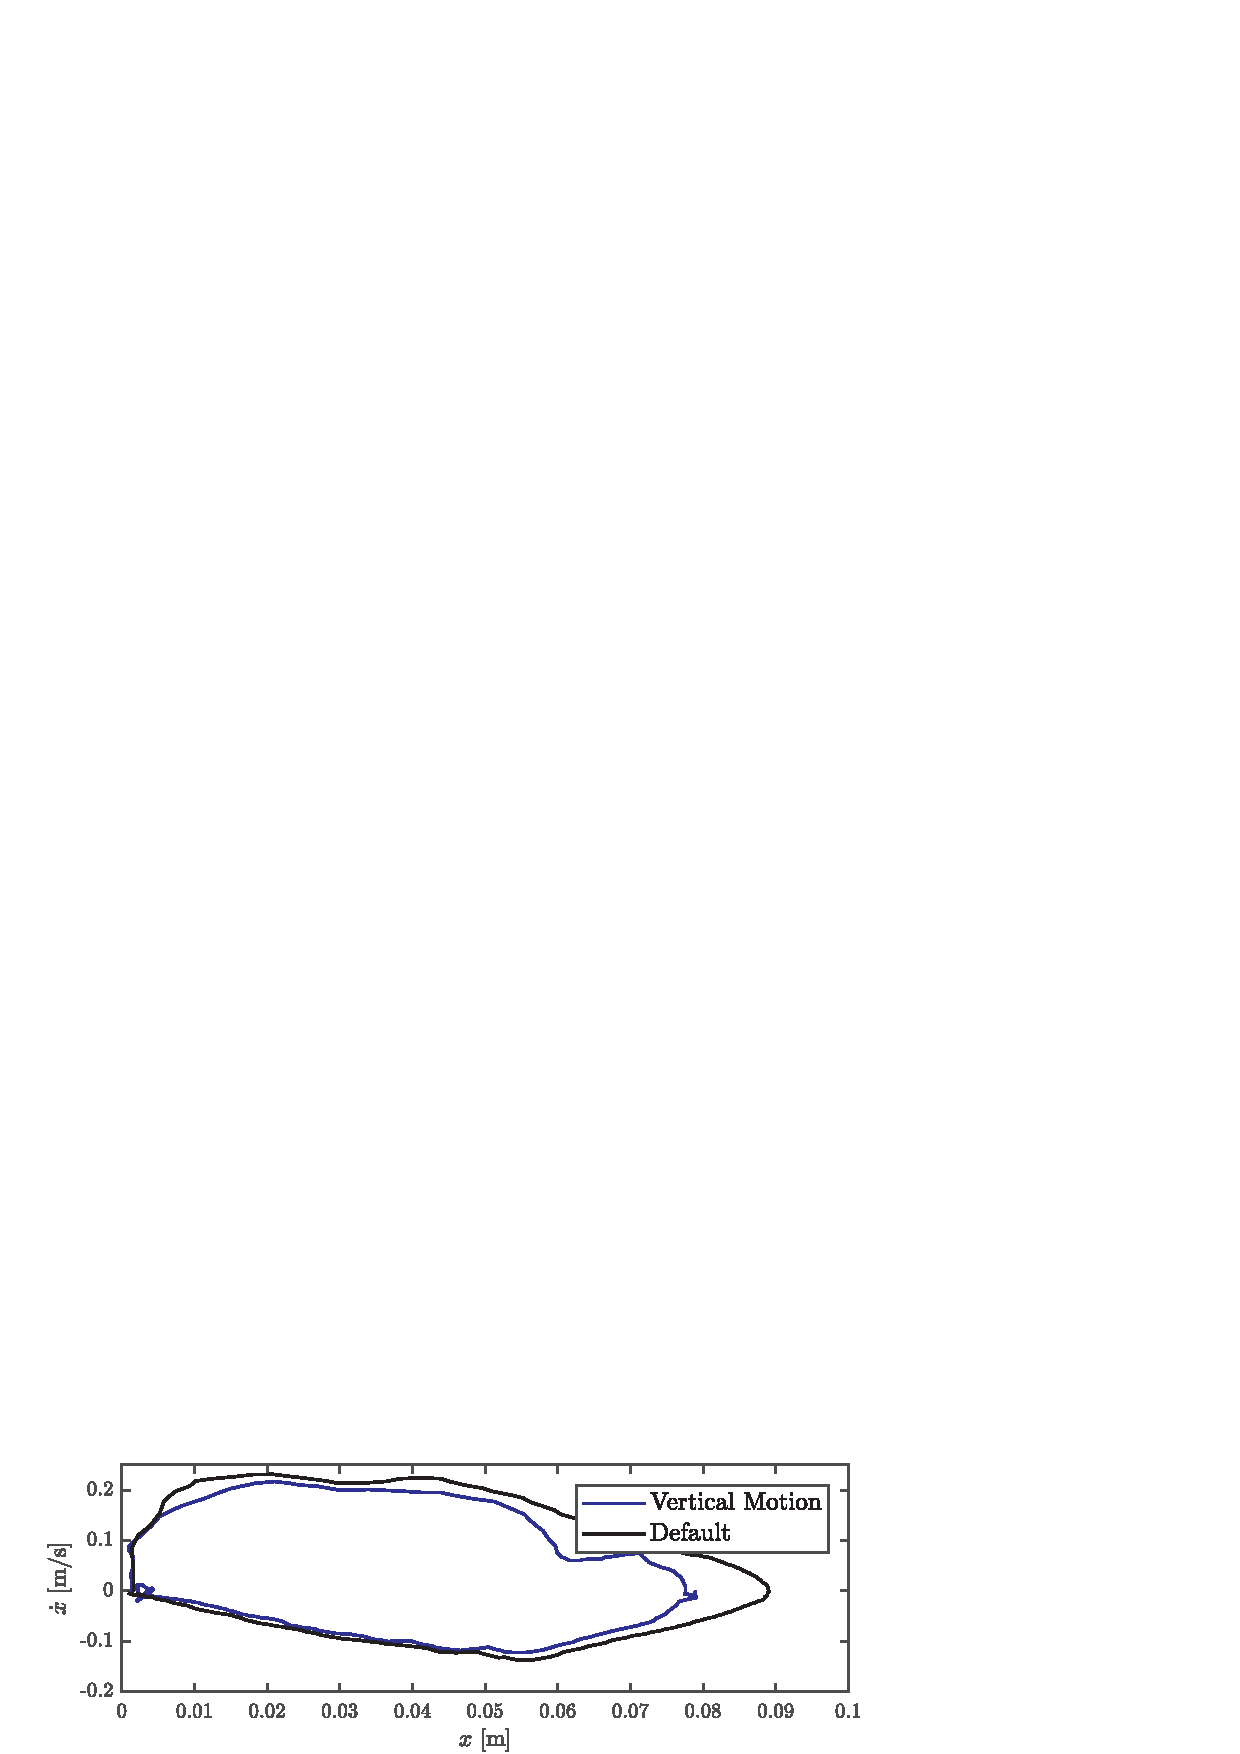
\includegraphics[width=3.3in]{valcomparephaseHW.png}
      \caption{Phase plot of push recovery on hardware. This is a pick of our data, where both pushes were of magnitude $33.2$ [Ns]. }
      \label{fig:valcomparephaseHW}
\end{figure}
\begin{figure}[h]
      \centering
      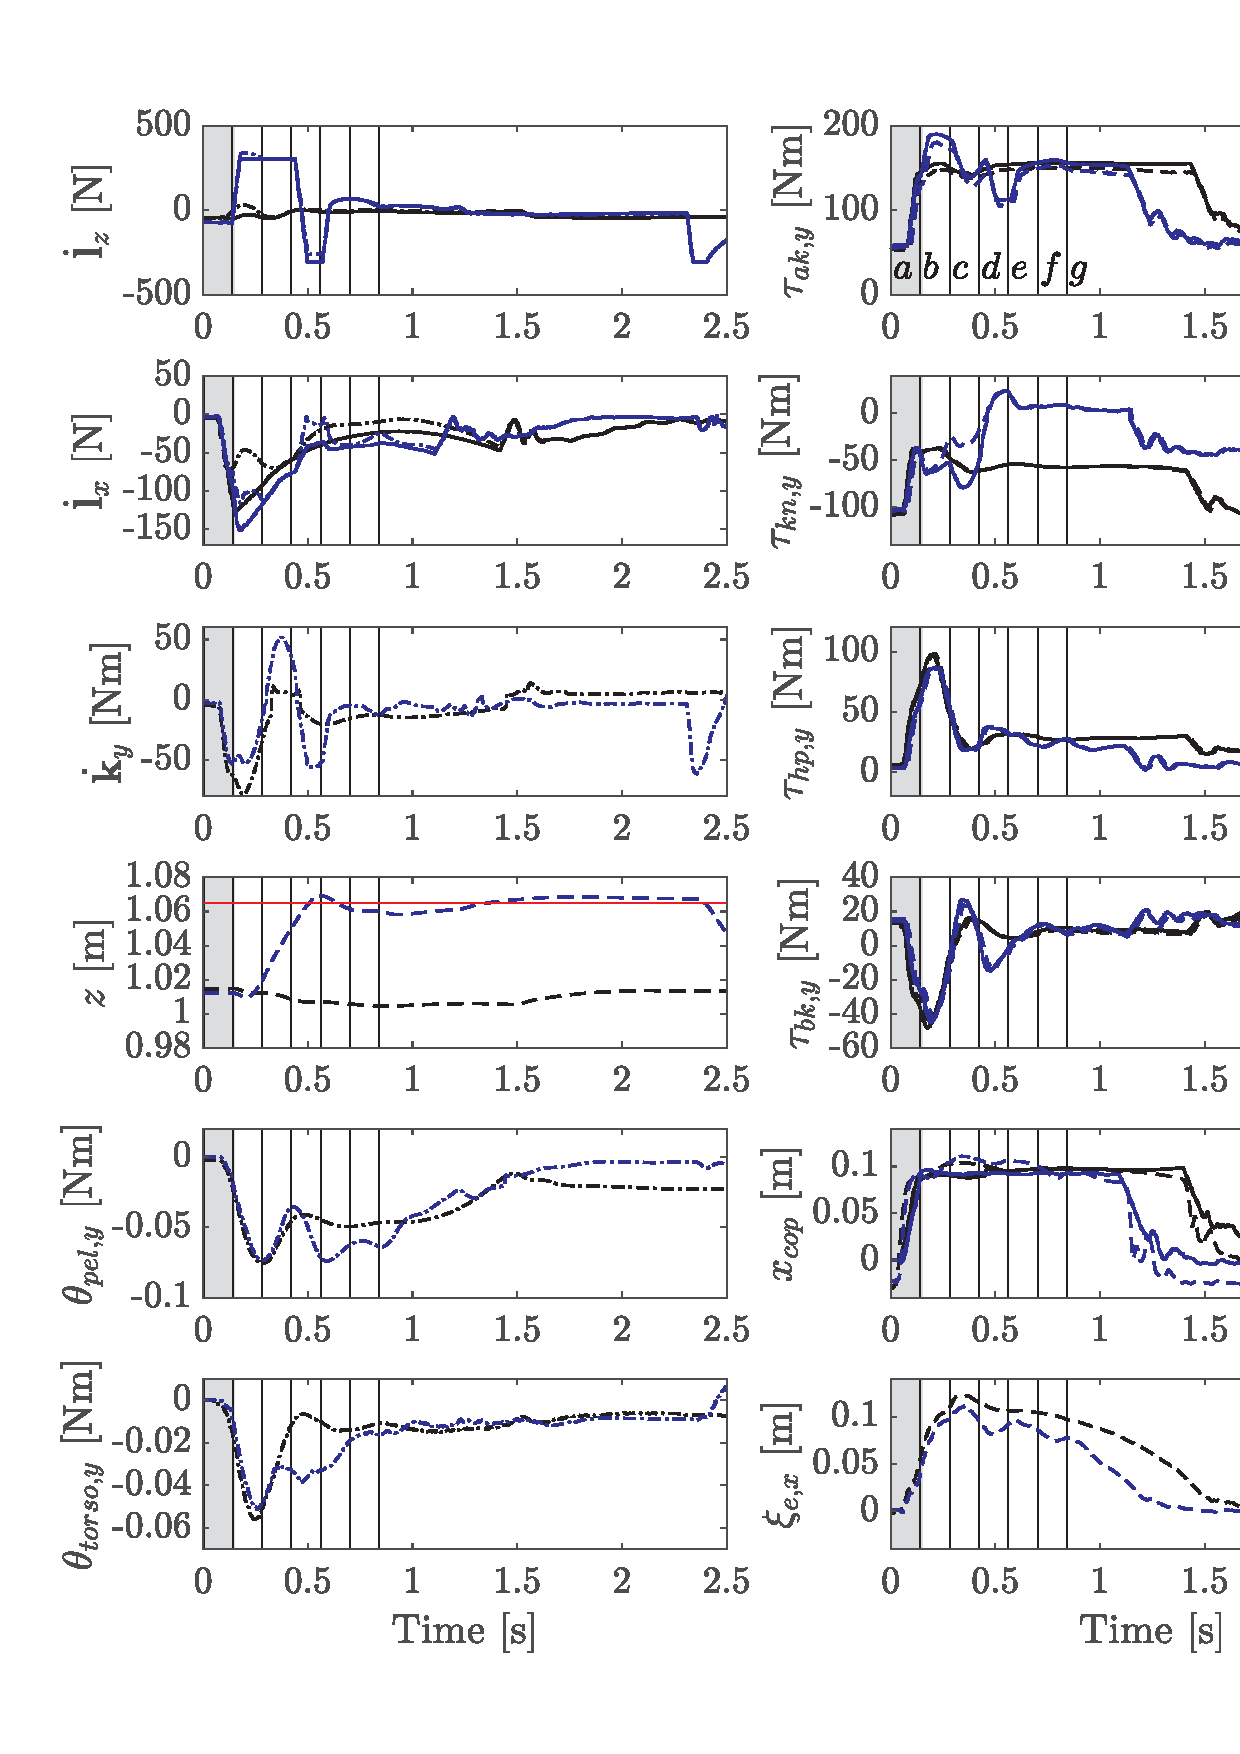
\includegraphics[width=3.3in]{valcomparetimeHW.png}
      \caption{Time plot of push recovery on hardware. This is a pick of our data, where both pushes were of magnitude $33.2$ [Ns]. $\boldmath{\tau}_{ak,y}$ is the average of the left and right ankle pitch torque. The letters next to the yellow lines match with the columns in Fig. \ref{fig:val}. }
      \label{fig:valcomparetimeHW}
\end{figure}
We tested the same two control setups on hardware as in simulation. We used a value of $\alpha_{\hat{\ddot{z}}_{c}}=0.8$, which appeared to be a better `estimate' for reaching the maximum height for the vertical motion controller.
\begin{figure*}[h]
\centering
  \begin{tabular}{ccccccc}
    \includegraphics[width=0.84in]{val1zr} &
    \includegraphics[width=0.84in]{val2zr} &
    \includegraphics[width=0.84in]{val3zr} &
    \includegraphics[width=0.84in]{val4z} &
    \includegraphics[width=0.84in]{val5z} &
    \includegraphics[width=0.84in]{val6z} &
    \includegraphics[width=0.84in]{val7z} ~\\[2ex]
     \includegraphics[width=0.84in]{val1dr} &
    \includegraphics[width=0.84in]{val2dr} &
    \includegraphics[width=0.84in]{val3dr} &
    \includegraphics[width=0.84in]{val4d} &
    \includegraphics[width=0.84in]{val5d} &
    \includegraphics[width=0.84in]{val6d} &
    \includegraphics[width=0.84in]{val7d} \\
    $a$&
    $b$&
    $c$&
    $d$&
    $e$&
    $f$&
    $g$\\
  \end{tabular}
  \caption{Time-lapse of Valkyrie recovering from a push using vertical motion (top row) and using the default controller setup (bottom row). The letters below the columns match with the letters next to the yellow lines in Fig. \ref{fig:valcomparetimeHW}. The push rod tip is encircled in red.}
  \label{fig:val}
\end{figure*}
We compared two times a dozen test samples that the robot `just' recovered from the applied push, which we define as the CoM coming closer than $5.0$ [mm] from the polygon edge. We measured the push force with an iLoad Pro Digital load sensor at its maximum record frequency of $100$ [Hz]. In Fig. \ref{fig:impulsecompare}, the average force profiles with standard deviation for both control setups are made visible, as well as an image of the load cell. The default setup still recovered with an average push of $35.3$ [Ns] and the vertical motion controller with $37.6$ [Ns], showing a slight robustness increase. The values for the integrated push force are very similar to the simulation results. However, the measured force profiles on hardware are different from the profile of the constant force applied in simulation.

We take an example case for comparison where the integrated push force on both setups was $33.2$ [Ns]. In Fig. \ref{fig:impulsecompare} the profiles for these two pushes are graphed. Note that this is a rough approximation of a similar disturbance, as other aspects like the force profile, record frequency and measurement noise of the load sensor also play a role in differences observed on the robot. In Fig \ref{fig:valcomparephaseHW}, a phase plot is shown for this push on both setups. 

In Fig. \ref{fig:valcomparetimeHW}, the same variables over time are shown as in the previous section. 
We found the differences in the length of each `bang' interesting, compared to simulation. This likely also is a reason why a higher value of $\alpha_{\hat{\ddot{z}}_{c}}$ was possible on hardware. Also notice the difference in resulting angular momentum rate. For this push on hardware, we measured $[-0.055,-0.074]$ radians of maximum pelvis and torso rotation error on the default setup and $[-0.045,-0.058]$ radians on the vertical motion controller, which is again less resulting body rotation with the vertical motion controller. The averaged ankle pitch torque over left and right is higher for the vertical motion controller, as expected. Also, the ankle torque of the vertical motion controller returns to steady-state earlier.

In Fig. \ref{fig:val}, two times a time-lapse image is shown of Valkyrie recovering from a push using the vertical motion controller, and using the default controller setup. The letters below the columns correspond with the numbers next to the yellow lines in Fig. \ref{fig:valcomparetimeHW}. Note how the contact of the push head is released, when the yellow lines are outside the gray area.

\section{CONCLUSION}\label{sec:conclusion}
To increase the reliability, it is important that humanoid robots improve their balancing behavior. In this paper we studied the effectiveness of vertical CoM motion in balance control. We derived capture regions for varying CoM height on a commonly used simple 2D model. We showed on Valkyrie in simulation and on hardware that balance can be improved using vertical CoM motions. Using this model-to-robot analysis, we showed differences that can be observed when going from a model-based expectation to the real result. 

For the future, we are interested in 3D and multi-step strategies for the robot to balance using CoM height variation. Also, we are interested in the coupled effects of e.g. combining vertical CoM motion with angular momentum strategies. We believe in building a portfolio of balancing strategies, as in \cite{griffin2017walking}, which can be used by the robot depending on the situation.


\addtolength{\textheight}{-0cm}   % This command serves to balance the column lengths
                                  % on the last page of the document manually. It shortens
                                  % the textheight of the last page by a suitable amount.
                                  % This command does not take effect until the next page
                                  % so it should come on the page before the last. Make
                                  % sure that you do not shorten the textheight too much.


\bibliographystyle{IEEEtran}
\bibliography{IEEEabrv,IEEEexample}



\end{document}
